\documentclass[__main__.tex]{subfiles}

\begin{document}

\qtitle{О}{09}
Временная и пространственная когерентность электромагнитных волн. Длина и радиус когерентности. Связь временной когерентности со степенью монохроматичности.\\ 

\begin{definition}
	Интерференцией называется взаимное увеличение(уменьшение) результирующей амплитуды двух или нескольких волн при их наложении друг на друга.
\end{definition}

\begin{definition}
	Два световых источника, способных создать интерференционную картину называются когерентными.
\end{definition}

Запишем формулу для интенсивности для случая общей схемы наблюдения интерференции с учетом оптической разности хода $\displaystyle \Delta = L_2 - L_1 = \frac{xa}{l}$:
\begin{gather*}
I = I_1 + I_2 + 2\sqrt{I_1 I_2}\cos\left(\frac{2\pi}{\lambda}\Delta\right) =
I_1 + I_2 + 2\sqrt{I_1 I_2}\cos\left(\frac{\pi x a}{\lambda l}\right),
\end{gather*}
для $I_1 = I_2 = I_0$:
\begin{gather}
\llabel{o-02-intensesch}
I = 2I_0\left(1 + \cos\left(\frac{2\pi}{\lambda}\Delta\right)\right) =
4I_0\cos^2\left(\frac{\pi xa}{\lambda l}\right),
\end{gather}

\begin{wrapfigure}{R}{0.3\linewidth}
	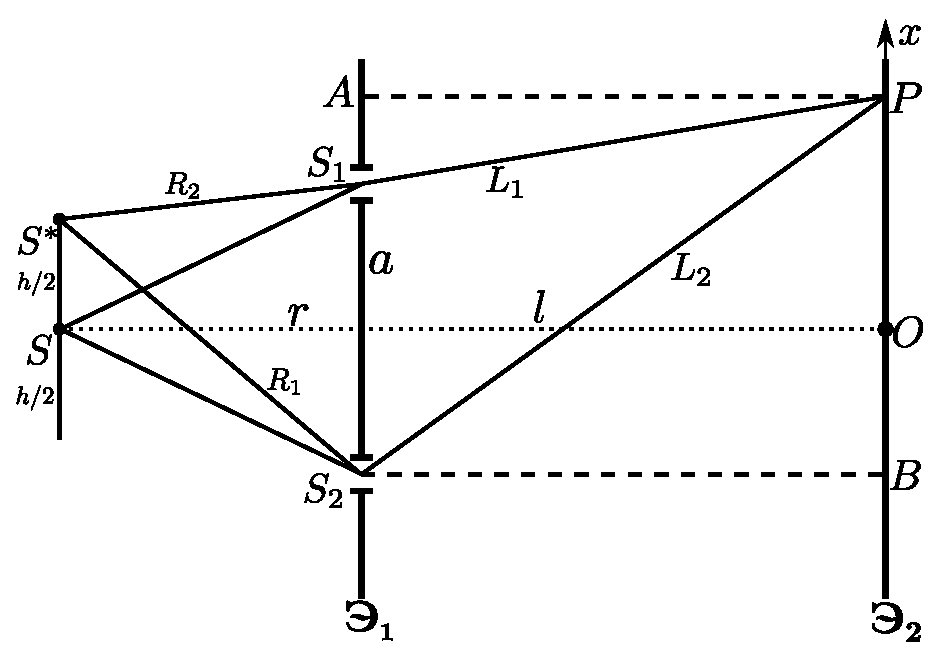
\includegraphics[width=1\linewidth]{img/o-09}{}
	\caption{}
	\llabel{o-01-prostra}
\end{wrapfigure}

\textbf{Пространственная когерентность.}
Рассмотрим общую схему интерференции с новым источником $S^*$, смещенными на $h/2$ относительно старого $S$ (см. Рис.01). Положим, что для расстояния до экрана $\text{Э}_1$ $r$ выполняется: $a\ll r, h\ll r$. Тогда аналогично предыдущему пункту получим добавочную разность хода до экрана $\text{Э}_1$: $\Delta^* = \frac{ha}{2r}$. 


Разность фаз для двух волн одной частоты с фазами $\varphi_1$ и $\varphi_2$ :
\begin{gather}
\llabel{o-02-phasediff}
\Delta \varphi = k(L_2 - L_1) = k \Delta =
(k = \frac{2\pi}{\lambda}) =
\frac{2\pi}{\lambda}\Delta,
\end{gather}
где $\Delta$ называется оптической разностью хода. 


Тогда добавочная разность фаз примет вид $\displaystyle\psi = \frac{2\pi}{\lambda}\Delta^*$, и перепишем (\lref{o-02-intensesch}):
\begin{gather}
\llabel{o-02-intensetwo}
I = 2I_0\left(1+\cos\left(\psi + \frac{2\pi}{\lambda}\Delta\right)\right),
\end{gather}

Теперь положим источник отрезком $[-h/2, h/2]$ и отыщем интенсивность, для этого усредним (\lref{o-02-intensetwo}) по фазе $\psi$ от $-\Delta\psi/2$ (нижний конец) до $\Delta\psi/2$ (верхний).
\begin{flalign*}
\begin{split}
\langle I \rangle &=
\frac{2I_0}{\Delta\psi}
\int\limits_{-\Delta\psi/2}^{\Delta\psi/2}
\left(
1 + \cos\left(\psi + \frac{2\pi}{\lambda}\Delta\right)
\right)d\psi = \\
&= 2I_0\left(
1 + \frac{2\sin(\Delta\psi/2)}{\Delta\psi}\cos\left(\frac{2\pi}{\lambda}\Delta\right)
\right) = \\
&= 2I_0\left(
1 + G(\Delta\psi)\cos\left(\frac{2\pi}{\lambda}\Delta\right)
\right),
\end{split}
\end{flalign*}
при $\Delta\psi \rightarrow 0$ $G(\Delta\psi) \rightarrow 1$ (первый замечательный предел), т.е получаем формулу (\lref{o-02-intensesch}) для точечного источника.
Отыщем значение $\Delta\psi$ при котором интерференционная картина пропадает. Это, очевидно, происходит при минимальном $\Delta\psi$ таком, что $G(\Delta\psi) = 0$. Т.е
\begin{flalign*}
\begin{split}
&\frac{\Delta\psi}{2} = \pi
\Rightarrow (\Delta\psi = \frac{2\pi}{\lambda}\frac{ha}{r}) \\ \Rightarrow
&\frac{\pi ha}{\lambda r} = \pi \Rightarrow a = \frac{\lambda r}{h},
\end{split}
\end{flalign*}
тогда для наблюдения пространственной интерференции должно выполняться условие 
$$
a < \frac{\lambda r}{h} = \rho_\text{ког}.
$$

\begin{definition}
	Величину $\displaystyle \rho_\text{ког} = \frac{\lambda r}{h}$ называют радиусом когерентности.
\end{definition}

\textbf{Временная когерентность.}
Рассмотрим не монохроматические лучи с частотами, лежащими в $\delta \omega$ окрестности $\omega$, где $|\delta \omega| \ll \omega$ (или с длинами волн в $U_{\delta \lambda}(\lambda)\colon |\delta \lambda| \ll \lambda$). Т.е. из
$\displaystyle\delta \phi = k \Delta = \frac{2\pi}{\lambda}\Delta$ можно сказать, что некоторые волны <<отстают по фазе>> от других.

\begin{definition}
	Световое излучение удовлетворяющее условию $\omega \in U_{\delta\omega}(\omega_0), |\delta\omega| \ll \omega$ называется квазимонохроматическим.
\end{definition}

Тогда для (\lref{o-02-intensesch}) пусть излучение источника $S$ имеет волновые числа в $(k_0-\delta k/2, k_0+\delta k/2)$ -- интервале шириной $\delta k$, из $\displaystyle k =\frac{2\pi}{\lambda}$ следует, что такое излучение квазимонохроматическое. Тогда из (\lref{o-02-intensesch}) найдем среднее значение интенсивности в этом случае.
\begin{flalign*}
\begin{split}
\langle I \rangle
&= \frac{2I_0}{\delta k}
\int\limits_{k_0-\delta k/2}^{k_0+\delta k/2}\left(1 + \cos(k \Delta)\right)dk = \\
&= 2I_0\left(
1 + \frac{2\sin(\Delta \delta k/2)}{\Delta \delta k}\cos(k_0 \Delta)
\right) = \\
&= 2I_0\left(1 + K(\delta k)\cos(k_0 \Delta)\right),
\end{split}
\end{flalign*}
Аналогично предыдущему пункту при $\delta k \rightarrow 0: K(\delta k) \rightarrow 1$ и интерференционная картина пропадет при 
$\delta k = \min\{\delta k\mid K(\delta k) = 0 \wedge \delta k \geq 0\}$ т.е. при 
$\Delta \delta k /2 = \pi$. Перепишем $\delta k$ через длину волны из $\displaystyle k =\frac{2\pi}{\lambda}$:
$$
\delta k = \frac{2\pi}{\lambda^2}\delta \lambda,
$$
минус, появившийся при дифференцировании уходит, т.к. все величины полагаются положительными.
Тогда условие наблюдения временной интерференции примет вид:
$$
\Delta < \frac{\lambda^2}{\delta \lambda} = l_\text{ког},
$$

Степень монохроматичности волны определяется шириной интервала длин волн (шириной спектра) 
$\delta \lambda$, отсюда и очевидна \textit{связь временной когерентности со степенью монохроматичности волны}.

\begin{definition}
	Величина $\displaystyle l_\text{ког} = \frac{\lambda^2}{\delta \lambda}$ называется длиной когерентности.
\end{definition}


\end{document}

